%chktex-file 1 chktex-file 2 chktex-file 3
%chktex-file 8 chktex-file 9 chktex-file 10
%chktex-file 13 %chktex-file 17 %chktex-file 23
%chktex-file 45 %chktex-file 25 %chktex-file 35
%chktex-file 40

\documentclass[oneside,12pt,a4paper]{report}

\usepackage{template}

\begin{document}

%    \begin{center}
%        \fontsize{17.28}{17.28}
%            \textbf{Equações Diferenciais Ordinárias}
%
%            \textbf{Banco de Questões}
%    \end{center}

%%%%%%%%%%%%%%%%%%%%%%%%%%%%%%%%%%%%%%%%%%%%%%%%%%%%%%%%%
% QUESTÕES
%%%%%%%%%%%%%%%%%%%%%%%%%%%%%%%%%%%%%%%%%%%%%%%%%%%%%%%%%

\chapter*{Capítulo 3}

    \exercicio[Zill, Seção 3.1, Exercício 12] O sudário de Turim mostra a imagem, em negativo, do corpo de um homem que aparentemente foi crucificado, e que muitos acreditam ser Jesus de Nazaré. Em 1988, o Vaticano deu a permissão para datar por carbono o sudário. Três laboratórios científicos e independentes analisaram o tecido e concluíram que o sudário tinha aproximadamente 660 anos, idade consistente com seu aparecimento histórico. Usando essa idade, determine a porcentagem da quantidade original de C-14 remanescente no tecido em 1988.

    \begin{resolucao}
        
    \end{resolucao}

    \exercicio[Zill, Seção 3.1, Exercício 18] Em $t=0$, um tubo de ensaio contendo um produto químico é imerso em um banho líquido. A temperatura inicial da substância química no tubo de ensaio é $80~^\circ F$. O banho de líquido tem uma temperatura controlada (medida em graus Fahrenheit) dada por $T_m=100-40e^{-0.1t},~t\geq0$, em que $t$ é medido em minutos.
    \begin{itensquestao}[1]
        \item Suponha que, dada a lei do aquecimento de Newton, $\dfrac{dT}{dt}=k(T-T_m)$, $k=-0.1$. Antes de resolver o PVI, descreva como você espera que a temperatura $T(t)$ do produto químico dentro do tubo de ensaio se comporte no curto prazo. E no longo prazo?
        \item Resolva o problema de valor inicial. Use um software para traçar o gráfico de $T(t)$ em intervalos de tempo de vários comprimentos. Os gráficos estão em acordo com as previsões realizadas no item anterior?
    \end{itensquestao}

    \begin{resolucao}
        
    \end{resolucao}

    \exercicio[Zill, Seção 3.1, Exercício 28] Suponha que, em um tanque em que é realizada uma mistura, a taxa na qual a salmoura é bombeada para o reservatório é de $3~\mathrm{gal/min}$ com concentração de $2~\mathrm{lb/gal}$, mas que a solução misturada é bombeada para fora a uma taxa de $2~\mathrm{gal/min}$. Uma vez que a salmoura está se acumulando no tanque a uma taxa de $1~\mathrm{gal/min}$, qualquer tanque finito deve, mais cedo ou mais tarde, derramar. Suponha que o tanque tenha uma tampa aberta e uma capacidade total de $400$ galões.
    \begin{itensquestao}[1]
        \item Quando o tanque transbordará?
        \item No instante em que estiver transbordando, qual será a quantidade de libras de sal no tanque?
        \item Suponha que, embora o tanque esteja transbordando, a solução salina continue a ser bombeada para dentro a uma taxa de $3~\mathrm{gal/min}$ e a solução bem misturada continue a ser bombeada para fora a uma taxa de $2~\mathrm{gal/min}$. Determine a quantidade de libras de sal no tanque no instante $t=150~\mathrm{min}$.
        \item Determine a quantidade de libras de sal no tanque quando $t\to\infty$.
        \item Use um software para obter o gráfico de $A(t)$ no intervalo $[0,500)$.
    \end{itensquestao}

    \begin{resolucao}
        
    \end{resolucao}

    \exercicio[Zill, Seção 3.1, Exercício 45] Um marca-passo cardíaco consiste de uma chave, uma bateria, um capacitor, e o coração como resistor. Quando a chave $S$ está em $P$, o capacitor se carrega. Já quando $S$ está em $Q$, o capacitor descarrega, enviando um estímulo elétrico para o coração. Durante esse tempo que o estímulo elétrico é aplicado para o coração, a tensão $E$ através do coração satisfaz a ED linear
    \[\frac{dE}{dt}=-\frac{1}{RC}E\]

    \begin{itensquestao}
        \item Vamos supor que, durante o intervalo de tempo $t_1$, $0<t<t_1$, a chave $S$ esteja na posição $P$ e o capacitor esteja sendo carregado. Quando a chave é movida para a posição $Q$ no instante $t_1$ o capacitor descarrega, enviando um impulso para o coração durante o intervalo de tempo $t_2$: $t_1\leq t<t_1+t_2$. Assim, durante o processo inicial de carregamento/descarregamento, $0<t<t_1+t_2$, a tensão para o coração é modelada pela equação diferencial definida por partes
        \begin{gather*}
            \frac{dE}{dt}=\begin{cases}
                0,\quad 0\leq t<t_1\\
                -\dfrac{1}{RC}E,\quad t_1\leq t<t_1+t_2
            \end{cases}
        \end{gather*}
        Movendo $S$ entre $P$ e $Q$, o carregamento e descarregamento em intervalos de tempo $t_1$ e $t_2$ é repetido indefinidamente. Suponha $t_1=4~s$, $t_2=2~s$, $E_0=12~V$, $E(0)=0$, $E(4)=12$, $E(6)=0$, $E(10)=12$, $E(12)=0$ e assim por diante. Resolva $E(t)$ para $0\leq t\leq24$.
        \item Suponha a título de ilustração que $R=C=1$. Use uma ferramenta gráfica para determinar a curva para o PVI no intervalo dado no item anterior.
    \end{itensquestao}

    \begin{figure}[H]
        \centering
        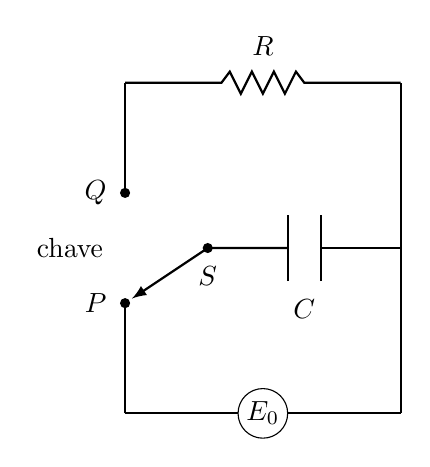
\begin{tikzpicture}[scale=0.7, >=latex, thick]

            % Coordenadas para os cantos do circuito principal
            \coordinate (BL) at (0,0); % Inferior Esquerdo
            \coordinate (BR) at (5,0); % Inferior Direito
            \coordinate (TL) at (0,6); % Superior Esquerdo
            \coordinate (TR) at (5,6); % Superior Direito

            % Coordenadas da chave
            \coordinate (P) at (0, 2);
            \coordinate (Q) at (0, 4);
            \coordinate (S) at (1.5, 3);

            % --- Fios Principais ---
            
            % Lado Esquerdo (interrompido pela chave)
            \draw (BL) -- (P);
            \draw (Q) -- (TL);
            
            % Lado Inferior (interrompido pela fonte E_0 centralizada em x=2.5)
            \draw (BL) -- (2.05, 0);
            \draw (2.95, 0) -- (BR);
            
            % Lado Direito
            \draw (BR) -- (TR);
            
            % Lado Superior (interrompido pelo resistor R centralizado em x=2.5)
            % Desenhando o resistor em zigue-zague
            \draw (TL) -- (1.75, 6) 
                -- (1.9, 6.2) -- (2.1, 5.8) 
                -- (2.3, 6.2) -- (2.5, 5.8) 
                -- (2.7, 6.2) -- (2.9, 5.8) 
                -- (3.1, 6.2) -- (3.25, 6) 
                -- (TR);
            
            % Fio horizontal do meio (interrompido pelo capacitor)
            % O segmento útil vai de x=1.5 até x=5. O centro é x=3.25.
            \draw (S) -- (2.95, 3);
            \draw (3.55, 3) -- (5, 3);

            % --- Componentes ---

            % Resistor R (rótulo)
            \node[above] at (2.5, 6.3) {$R$};

            % Capacitor C (centralizado no fio do meio)
            \draw (2.95, 2.4) -- (2.95, 3.6);
            \draw (3.55, 2.4) -- (3.55, 3.6);
            \node at (3.25, 1.9) {$C$};

            % Fonte de Tensão E_0 (centralizada no fio de baixo)
            \draw[fill=white, thin] (2.5, 0) circle (0.45);
            \node at (2.5, 0) {$E_0$};

            % Elementos da Chave (P, Q, S)
            \filldraw (P) circle (2pt) node[left=3pt] {$P$};
            \filldraw (Q) circle (2pt) node[left=3pt] {$Q$};
            \filldraw (S) circle (2pt) node[below=3pt] {$S$};
            
            \node at (-1.0, 3) {chave};
            
            % Braço móvel da chave (de S para P)
            \draw[->, shorten >=3pt] (S) -- (P);

        \end{tikzpicture}
    \end{figure}

    \begin{resolucao}
        
    \end{resolucao}

    \exercicio[Zill, Seção 3.1, Exercícios 46, 47 (a)] Uma caixa de massa $m$ desliza por um plano inclinado de ângulo $\theta$ com a horizontal, conforme a figura abaixo.

    \begin{figure}[H]
        \centering
        \begin{tikzpicture}[>=stealth, scale=0.8]
            % Parâmetros do plano inclinado
            \pgfmathsetmacro{\angle}{30} % Ângulo de inclinação theta
            \pgfmathsetmacro{\base}{8}   % Comprimento da base
            \pgfmathsetmacro{\height}{\base*tan(\angle)} % Altura

            % Chão (sombreado e linha)
            \fill[gray!20] (-0.3,-0.15) rectangle (\base+0.3, 0);
            \draw[thick, gray!70!black] (-0.3,0) -- (\base+0.3,0);

            % Triângulo do plano inclinado
            \draw[thick] (0,0) -- (\base,0) -- (\base,\height) -- cycle;

            % Ângulo theta
            \draw (1,0) arc (0:\angle:1);
            \node at (\angle/2:1.3) {$\theta$};

            % Coordenadas para o bloco (centro da base do bloco)
            \pgfmathsetmacro{\px}{4.2}
            \pgfmathsetmacro{\py}{\px*tan(\angle)}
            \coordinate (P) at (\px,\py);

            % Bloco
            \begin{scope}[shift={(P)}, rotate=\angle]
                \draw[fill=gray!50, draw=gray!70!black, thick, rounded corners=0.5pt] (-0.75,0) rectangle (0.75, 1.2);
            \end{scope}

            % Vetor Peso (W)
            \def\wlen{2}
            \coordinate (W) at ($(P) + (0,-\wlen)$);

            % Projeções tracejadas do peso (componentes x e y)
            \coordinate (Incline) at ($(P) + (\angle:1)$);
            \coordinate (Perp) at ($(P) + (\angle-90:1)$);
            \coordinate (Wpar) at ($(P)!(W)!(Incline)$);
            \coordinate (Wperp) at ($(P)!(W)!(Perp)$);

            % Linhas tracejadas formando o retângulo das componentes
            \draw[dashed, thick] (P) -- (Wperp) -- (W) -- (Wpar);

            % Vetores de Força e Movimento
            % Força de atrito
            \draw[->, line width=1.5pt, gray!80!black] (P) -- ++(\angle:2) node[pos=0.8, below right, text=black] {atrito};

            % Sentido do movimento
            \draw[->, line width=1.5pt, gray!80!black] (P) -- ++(180+\angle:2) node[pos=0.6, above left, text=black] {movimento};

            % Linha do vetor peso
            \draw[->, line width=1.5pt, blue!75!black] (P) -- (W);

            % Rótulo "W = mg" com seta apontando para o vetor
            \node[right] (Wlabel) at ($(P) + (1.2, -1.5)$) {$W = mg$};
            \draw[->, thin] (Wlabel.west) -- ($(P)!0.47!(W)$);

            % Ponto central (desenhado por último para ficar sobre as linhas)
            \fill (P) circle (2.5pt);

            % Indicador de altura no lado direito (50 pés)
            \draw (\base+0.2, 0) -- (\base+0.6, 0);
            \draw (\base+0.2, \height) -- (\base+0.6, \height);
            \draw[<->] (\base+0.4, 0) -- (\base+0.4, \height) node[midway, fill=white, inner sep=2pt] {50 pés};

        \end{tikzpicture}
    \end{figure}

    \begin{itensquestao}
        \item Encontre uma equação diferencial para a velocidade $v(t)$ da caixa no instante $t$ em cada um dos três casos seguintes:
        \begin{enumerate}[label=\roman*)]
            \item Ausência de atrito e resistência do ar
            \item Com atrito e ausência de resistência do ar
            \item Com atrito e resistência do ar
        \end{enumerate}
        Nos casos (i) e (ii), use o fato de que a força de atrito que se opõe ao movimento da caixa é $\mu N$, onde $\mu$ é o coeficiente de atrito de deslizamento e $N$ é o componente normal do peso da caixa. No caso (iii), assuma que a resistência do ar é proporcional à velocidade instantânea.

        \item Na parte (a), suponha que a caixa pesa $96~\mathrm{lb}$, que $\theta=30^\circ$, que $\mu=\dfrac{\sqrt{3}}{4}$ e que a força de resistência do ar é numericamente igual a $\dfrac{v}{4}$. Resolva a equação diferencial em cada um dos três casos, assumindo que a caixa começa a partir do repouso no ponto mais alto, $50~\mathrm{ft}$ acima do solo.
        
        \item Sendo $\mu=\dfrac{\sqrt{3}}{4}$ e $\theta=23^\circ$, estime, a partir do modelo (ii), a menor velocidade inicial $v_0$ que a caixa deve ter para, iniciando do ponto mais alto ($50~\mathrm{ft}$ acima do chão), escorregar completamente no plano inclinado. Encontre ainda o tempo total desse movimento.
    \end{itensquestao}

    \begin{resolucao}
        
    \end{resolucao}

    \exercicio[Zill, Seção 3.2, Exercício 5]
        \begin{itensquestao}
            \item Se um número constante $h$ de peixes é removido de um pesqueiro por unidade de tempo, então um modelo para a população $P(t)$ do pesqueiro em um instante de tempo $t$ é dado por
            $$ \frac{dP}{dt} = P(a - bP) - h, \quad P(0) = P_0, $$
            em que $a, b, h$ e $P_0$ são constantes positivas. Suponha que $a = 5, b = 1$ e $h = 4$. Uma vez que a ED é autônoma, utilize o conceito de fase para esboçar curvas solução representativas dos três casos $P_0 > 4$, $1 < P_0 < 4$ e $0 < P_0 < 1$. Determine o comportamento a longo prazo da população em cada caso.
            \item Resolva o PVI da parte (a). Verifique os resultados do seu gráfico de fase na parte (a) usando um software para determinar um gráfico de $P(t)$ com condições iniciais tomadas de cada um dos três intervalos dados.
            \item Use os resultados das partes (a) e (b) para determinar se a população de peixes é extinta em um tempo finito. Em caso positivo, encontre esse tempo.
        \end{itensquestao}
    \begin{resolucao}
        
    \end{resolucao}

    \exercicio[Zill, Seção 3.2, Exercício 9] Duas substâncias químicas, $A$ e $B$, são combinadas para formar uma substância química $C$. A taxa ou velocidade de reação é proporcional ao produto da quantidade instantânea de $A$ e $B$ não convertida na substância $C$. Inicialmente, há $40$ g de $A$ e $50$ g de $B$, e para cada grama de $B$ são usados $2$ g de $A$. É observado que em $5$ minutos são formados $10$ g de $C$. Quanto será formado em $20$ minutos? Qual será a quantidade limite de $C$ após um longo período? Quanto resta das substâncias $A$ e $B$ após um longo período?

    \begin{resolucao}
        
    \end{resolucao}

    \exercicio[Zill, Seção 3.2, Exercício 18] A equação diferencial
    $$ \frac{dy}{dx} = \frac{-x + \sqrt{x^2+y^2}}{y} $$
    descreve a forma de uma curva plana $C$ que refletirá para o mesmo ponto todos os feixes de luz incidentes e poderia ser um modelo para o espelho de um telescópio refletivo, uma antena de um satélite ou um coletor solar.
        \begin{itensquestao}
            \item Verifique que a equação diferencial é homogênea. Mostre que a substituição $y = ux$ dá lugar a
            $$ \frac{u \, du}{\sqrt{1+u^2}(1 - \sqrt{1+u^2})} = \frac{dx}{x}. $$
            Use uma substituição para integrar o lado esquerdo da equação. Mostre que a curva $C$ deve ser uma parábola com o foco na origem e simétrica em relação ao eixo $x$.
            \item Mostre que a primeira equação diferencial pode também ser resolvida por meio da substituição $u = x^2 + y^2$.
        \end{itensquestao}

    \begin{resolucao}
        
    \end{resolucao}

    \exercicio[Zill, Seção 3.2, Exercício 20] Um lago decorativo em Palm Springs, Califórnia, tem a forma de um tanque hemisférico que deve ser enchido com água bombeada por meio de um orifício no fundo do tanque. Suponha que o raio do tanque seja $R = 10~\mathrm{ft}$, a água seja bombeada a uma taxa de $\pi~\mathrm{ft^3/min}$ e que o tanque esteja inicialmente vazio. À medida que o tanque é enchido, a água evapora. Suponha que a taxa de evaporação seja proporcional à área $A$ da superfície da água e que a constante de proporcionalidade seja igual a $k = 0,01$.

    \begin{figure}[H]
        \centering
        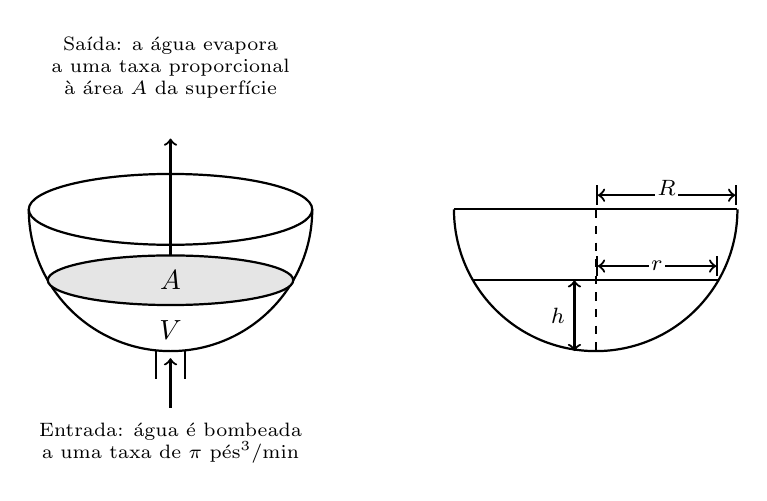
\begin{tikzpicture}[scale=0.9]
            % --- Parte A: Tanque Hemisférico ---
            \begin{scope}[shift={(0,0)}]
                % Textos superiores
                \node[align=center, font=\scriptsize] at (0, 2) {Saída: a água evapora \\ a uma taxa proporcional \\ à área $A$ da superfície};
                
                % Setas de evaporação
                \draw[->, thick] (0, -1) -- (0, 1);
                
                % Elipse superior (borda do tanque)
                \draw[thick] (0,0) ellipse (2cm and 0.5cm);
                
                % Arco do tanque (hemisfério)
                \draw[thick] (-2,0) arc (180:360:2cm);
                
                % Superfície da água
                \draw[thick, fill=gray!20] (0,-1) ellipse (1.732cm and 0.35cm);
                \node at (0, -1) {$A$};
                \node at (0, -1.7) {$V$};
                
                % Tubo de entrada de água (fundo)
                \draw[thick] (-0.2,-2) -- (-0.2,-2.4);
                \draw[thick] (0.2,-2) -- (0.2,-2.4);
                \draw[->, thick] (0,-2.8) -- (0,-2.1);
                
                % Texto inferior (Entrada)
                \node[align=center, font=\scriptsize] at (0, -3.3) {Entrada: água é bombeada \\ a uma taxa de $\pi$ pés$^3$/min};
            \end{scope}

            % --- Parte B: Seção Transversal ---
            \begin{scope}[shift={(6,0)}]
                % Borda superior e arco do tanque
                \draw[thick] (-2,0) -- (2,0);
                \draw[thick] (-2,0) arc (180:360:2cm);
                
                % Nível da água
                \draw[thick] (-1.732,-1) -- (1.732,-1);
                
                % Eixo central tracejado
                \draw[dashed, thick] (0,0) -- (0,-2);
                
                % Raio R
                \draw[|<->|, thick] (0,0.2) -- (2,0.2);
                \node[font=\footnotesize, fill=white, inner sep=1pt] at (1, 0.3) {$R$};
                
                % Raio r (superfície da água)
                \draw[|<->|, thick] (0,-0.8) -- (1.732,-0.8);
                \node[font=\footnotesize, fill=white, inner sep=1pt] at (0.866, -0.8) {$r$};
                
                % Altura h
                \draw[<->, thick] (-0.3,-1) -- (-0.3,-2);
                \node[font=\footnotesize, left] at (-0.3, -1.5) {$h$};
            \end{scope};

        \end{tikzpicture}
    \end{figure}

    \begin{itensquestao}
        \item A taxa de variação $dV/dt$ do volume de água no instante $t$ é uma taxa líquida. Use esta taxa líquida para determinar uma equação diferencial para a altura $h$ da água no instante $t$. O volume de água mostrado na figura é $V = \pi Rh^2 - \dfrac{1}{3}\pi h^3$, onde $R = 10$. Expresse a área da superfície da água $A = \pi r^2$ em termos de $h$.
        \item Resolva a equação diferencial do item (a). Faça o gráfico da solução.
        \item Se não houvesse evaporação, quanto tempo levaria para o tanque ficar cheio?
        \item Com a evaporação, qual será a profundidade da água no instante encontrado no item (c)? O tanque chegará a encher? Prove sua afirmativa.
    \end{itensquestao}

    \begin{resolucao}
        
    \end{resolucao}

\chapter*{Capítulo 4}

\section*{Variação dos Parâmetros (Seção 4.6)}

\exercicio[Zill, Seção 4.6, Exercícios 9, 12, 15, 17 e 21] Resolva cada equação diferencial por variação dos parâmetros, respeitando as condições iniciais quando houver.
\begin{itensquestao}[2]
    \item $y''-4y=\dfrac{e^{2x}}{x}$
    \item $y''-2y'+y=\dfrac{e^{x}}{1+x^2}$
    \item $y''+2y'+y=e^{-t}\ln(t)$
    \item $3y''-6y'+6y=e^x\sec(x)$
    \item $y''+2y'-8y=2e^{-2x}-e^{-x},\\ y(0)=1,~y'(0)=0$
\end{itensquestao}

\begin{resolucao}
    \itemresolucao Primeiramente, devemos resolver a equação homogênea auxiliar $y''-4y=0$. Sua equação característica é $\lambda^2-4=0$, por meio da qual obtemos $\lambda=\pm2$. Ou seja, as soluções que satisfazem a equação homogênea são $y_1(x) = e^{2x}$ e $y_2(x) = e^{-2x}$. Podemos escrever a solução da equação homogênea como uma combinação linear de $y_1$ e $y_2$, da forma
    \[y_h(x)=c_1e^{2x}+c_2e^{-2x}\]

    Em seguida, prosseguimos com a determinação da solução particular. Em um primeiro momento, calculamos o Wronskiano das soluções:
    \[W(x)=\begin{vmatrix}
        e^{2x} & e^{-2x}\\
        2e^{2x} & -2e^{-2x}
    \end{vmatrix}=-2-2=-4\]

    Além disso,
    \[W_1(x)=\begin{vmatrix}
        0 & e^{-2x}\\
        1 & -2e^{-2x}
    \end{vmatrix}=-e^{-2x}\quad e \quad W_2(x)=\begin{vmatrix}
        e^{2x}  & 0\\
        2e^{2x} & 1
    \end{vmatrix}=e^{2x}\]

    Dessa forma, segue da fórmula de variação de parâmetros que
    \[y_p(x)=\sum_{i=1}^{2}y_i\int\frac{f(x)W_i(x)}{W(x)}dx, \text{ onde } f(x)=\frac{e^{2x}}{x}\]
    \[y_p(x)=e^{2x}\int\frac{e^{2x}(-e^{-2x})}{4x}dx+e^{-2x}\int\frac{e^{2x}e^{2x}}{4x}dx\]
    \[y_p(x)=-\frac{e^{2x}}{4}\int\frac{1}{x}dx+\frac{e^{-2x}}{4}\int\frac{e^{4x}}{x}dx\]

    Enquanto a primeira integral é direta, a segunda é não elementar. Dessa forma, vamos expressá-la por meio da variável muda $t$. Além disso, tomamos um intervalo que não engloba a descontinuidade em $x=0$:
    \[y_p(x)=-\frac{e^{2x}}{4}\ln(x)+\frac{e^{-2x}}{4}\int_{x_0}^{x}\frac{e^{4t}}{t}dt;\quad x_0>0\]

    Temos que $y(x)=y_h(x)+y_p(x)$. Assim,
    \[\boxed{y(x)=c_1e^{2x}+c_2e^{-2x}-\frac{e^{2x}}{4}\ln(x)+\frac{e^{-2x}}{4}\int_{x_0}^{x}\frac{e^{4t}}{t}dt;\quad x_0>0}\]

    \itemresolucao Tomando a equação característica da equação homogênea auxiliar, 
    \[\lambda^2-2\lambda+1=0\Rightarrow(\lambda-1)^2=0\Rightarrow\lambda=1\]
    Como a equação tem raízes repetidas, a fim de encontrar soluções linearmente independentes, temos $y_1=e^x$ e $y_2=xe^x$. Assim, a solução da equação homogênea será uma combinação linear de $y_1$ e $y_2$, da forma
    \[y_h=c_1e^x+c_2xe^x\]
    Calculando o Wronskiano das soluções,
    \[W(x)=\begin{vmatrix}
        e^{x} & xe^{x}\\
        e^{x} & e^{x}(x+1)
    \end{vmatrix}=e^{2x}(1+x)-xe^{2x}=e^{2x}\]

    Além disso,
    \[W_1(x)=\begin{vmatrix}
        0 & xe^{x}\\
        1 & e^{x}(x+1)
    \end{vmatrix}=-xe^{x}\quad e \quad W_2(x)=\begin{vmatrix}
        e^{x}  & 0\\
        e^{x} & 1
    \end{vmatrix}=e^{x}\]

    Segue de fórmula de variação dos parâmetros que
    \[y_p(x)=\sum_{i=1}^{2}y_i\int\frac{f(x)W_i(x)}{W(x)}dx, \text{ onde } f(x)=\frac{e^{x}}{1+x^2}\]
    \[y_p(x)=e^x\int\frac{\frac{e^x}{1+x^2}(-xe^x)}{e^{2x}}dx+xe^x\int\frac{\frac{e^x}{1+x^2}(e^x)}{e^{2x}}dx\]
    \[y_p(x)=-e^x\int\frac{x}{1+x^2}dx+xe^x\int\frac{1}{1+x^2}dx\]
    \[y_p(x)=-\frac{e^x}{2}\ln(1+x^2)+xe^x\arctan(x)\]

    Assim, a solução geral da equação diferencial é dada por $y(x)=y_h(x)+y_p(x)$,
    \[\boxed{y(x)=c_1e^x+c_2xe^x+e^x\left(x\arctan(x)-\frac{\ln(1+x^2)}{2}\right)}\]

    \itemresolucao Resolvendo a equação característica da homogênea auxiliar,
    \[\lambda^2+2\lambda+1=0\Rightarrow(\lambda+1)^2\Rightarrow\lambda=-1\]
    Dessa forma, tomando soluções linearmente independentes, temos $y_1=e^{-t}$ e $y_2=te^{-t}$. Ou seja, a solução da equação homogênea formada pela combinação linear de $y_1$ e $y_2$ é
    \[y_h(t)=c_1e^{-t}+c_2te^{-t}\]

    Partindo para a determinação da solução particular por meio da variação de parâmetros, calculamos o Wronskiano:
    \[W(t)=\begin{vmatrix}
        e^{-t} & te^{-t}\\
        -e^{-t} & e^{-t}(1-t)
    \end{vmatrix}=e^{-2t}(1-t)+te^{-2t}=e^{-2t}\]

    Ademais,
    \[W_1(t)=\begin{vmatrix}
        0 & te^{-t}\\
        1 & e^{-t}(1-t)
    \end{vmatrix}=-te^{-t}\quad e \quad W_2(t)=\begin{vmatrix}
        e^{-t}   & 0\\
        -e^{-t} & 1
    \end{vmatrix}=e^{-t}\]

    Dessa forma, segue que
    \[y_p(t)=e^{-t}\int\frac{e^{-t}\ln(t)(-te^{-t})}{e^{-2t}}dt+te^{-t}\int\frac{e^{-t}\ln(t)e^{-t}}{e^{-2t}}dt\]
    \[y_p(t)=-e^{-t}\int t\ln(t)dt+te^{-t}\int\ln(t)dt\]
    Calcularemos as duas integrais por partes. Para a primeira, tomamos $\ln(t)=u\rightarrow1/t~dt=du$ e $t~dt=dv\rightarrow t^2/2=v$. Já para a segunda, temos $\ln(t)=u\rightarrow1/t~dt=du$ e $dt=dv\rightarrow t=v$. Nesse sentido,
    \[y_p(t)=-e^{-t}\left[\frac{t^2}{2}\ln(t)-\int\frac{t}{2}dt\right]+te^{-t}\left[t\ln(t)-\int dt\right]\]
    \[y_p(t)=-e^{-t}\left[\frac{t^2}{2}\ln(t)-\frac{t^2}{4}\right]+te^{-t}\left[t\ln(t)-t\right]=e^{-t}\left[\frac{t^2}{2}\ln(t)-\frac{3}{4}t^2\right]\]

    Assim, a solução geral da equação é
    \[\boxed{c_1e^{-t}+c_2te^{-t}+e^{-t}\left[\frac{t^2}{2}\ln(t)-\frac{3}{4}t^2\right]}\]

    \itemresolucao Primeiramente, devemos reescrever a equação diferencial na forma padrão:
    \[y''-2y'+2=\frac{e^x\sec(x)}{3}\]
    Resolvendo a equação característica da homogênea auxiliar,
    \[\lambda^2-2\lambda+2=0\Rightarrow\lambda_{1,2}=\frac{2\pm\sqrt{2^2-4\cdot1\cdot2}}{2}\Rightarrow\lambda_{1,2}=1\pm i\]

    Tomando $\lambda=1+i$, temos que as soluções reaisi linearmente independentes da equação são $y_1=e^x\cos(x)$ e $y_2=e^x\sin(x)$. Ou seja, uma combinação linear dessas duas soluções é
    \[y_h(x)=c_1e^x\cos(x)+c_2e^x\sin(x)\]

    Calculemos o Wronskiano das soluções:
    \[W(x)=\begin{vmatrix}
        e^{x}\cos(x) & e^{x}\sin(x)\\
        e^{x}(\cos(x)-\sin(x)) & e^{x}(\sin(x)+\cos(x))
    \end{vmatrix}=e^{2x}\]

    Ademais,
    \[W_1(x)=\begin{vmatrix}
        0 & e^{x}\sin(x)\\
        1 & e^{x}(\sin(x)+\cos(x))
    \end{vmatrix}=-e^{x}\sin(x)\] 
    \[W_2(x)=\begin{vmatrix}
        e^{x}\cos(x) & 0\\
        e^{x}(\cos(x)-\sin(x)) & 1
    \end{vmatrix}=e^{x}\cos(x)\]

    A partir da fórmula de variação dos parâmetros,
    \[y_p(x)=e^x\cos(x)\int\frac{\frac{e^x\sec(x)}{3}(-e^x\sin(x))}{e^{2x}}dx+e^x\sin(x)\int\frac{\frac{e^x\sec(x)}{3}(e^x\cos(x))}{e^{2x}}dx\]
    \[y_p(x)=-\frac{e^x\cos(x)}{3}\int\frac{\sin(x)}{\cos(x)}dx+\frac{e^x\sin(x)}{3}\int dx\]
    \[y_p(x)=\frac{e^x}{3}(\cos(x)\ln|\cos(x)|+x\sin(x))\]

    Ou seja, a solução geral da equação diferencial é
    \[\boxed{y(x)=c_1e^x\cos(x)+c_2e^x\sin(x)+\frac{e^x}{3}(\cos(x)\ln|\cos(x)|+x\sin(x))}\]

    \itemresolucao Resolvendo a equação homogênea associada,
    \[\lambda^2+2\lambda-8=0\Rightarrow(\lambda-2)(\lambda+4)=0\Rightarrow\lambda=2\text{ ou }\lambda=-4\]

    Nesse sentido, são soluções linearmente independentes da homogênea associada $y_1=e^{2x}$ e $y_2=e^{-4x}$, com $y_h=c_1e^{2x}+c_2e^{-4x}$. Calculando o Wronskiano dessas soluções,
    \[W(x)=\begin{vmatrix}
        e^{2x} & e^{-4x}\\
        2e^{2x} & -4e^{-4x}
    \end{vmatrix}=-6e^{-2x}\]

    Além disso,
    \[W_1(x)=\begin{vmatrix}
        0 & e^{-4x}\\
        1 & -4e^{-4x}
    \end{vmatrix}=-e^{-4x}\quad e \quad W_2(x)=\begin{vmatrix}
        e^{2x}  & 0\\
        2e^{2x} & 1
    \end{vmatrix}=e^{2x}\]

    Da fórmula de variação dos parâmetros,
    \[y_p(x)=e^{2x}\int\frac{(2e^{-2x}-e^{-x})(-e^{-4x})}{-6e^{-2x}}dx+e^{-4x}\int\frac{(2e^{-2x}-e^{-x})(e^{2x})}{-6e^{-2x}}dx\]
    \[y_p(x)=\frac{1}{9}e^{-x}-\frac{1}{4}e^{-2x}\]

    Assim, a solução geral da equação diferencial é
    \[\boxed{c_1e^{2x}+c_2e^{-4x}+\frac{1}{9}e^{-x}-\frac{1}{4}e^{-2x}}\]

    Agora, a fim de resolver o PVI, devemos substituir as condições iniciaisi fornecidas:
    \[y(0)=1\Rightarrow c_1+c_2-\frac{5}{36}=1\Rightarrow c_1+c_2=\frac{41}{36}\]
    \[y'(0)=0\Rightarrow 2c_1-4c_2-\frac{1}{9}+\frac{1}{2}=0\Rightarrow c_1-2c_2=-\frac{7}{36}\]

    Dessa forma, temos um sistema em $c_1$ e $c_2$:
    \[\begin{cases}
        c_1+c_2=\frac{41}{36}\\
        c_1-2c_2=-\frac{7}{36}
    \end{cases}\]
    Resolvendo esse sistema, encontramos $c_1=\frac{25}{36}$ e $c_2=\frac{4}{9}$. Ou seja, a solução geral do PVI é dada por
    \[\boxed{\frac{25}{36}e^{2x}+\frac{4}{9}e^{-4x}+\frac{1}{9}e^{-x}-\frac{1}{4}e^{-2x}}\]

\end{resolucao}

\exercicio[Zill, Seção 4.6, Exercício 23] As funções indicadas são soluções linearmente independentes da equação diferencial homogênea associada em $(0,\infty)$. Ache a solução geral da equação não homogênea dada:
\[x^2y''+xy'+\left(x^2-\frac{1}{4}\right)y=x^\frac{3}{2};\quad y_1=x^{-\frac{1}{2}}\cos(x),~y_2=x^{-\frac{1}{2}}\sin(x)\]

\begin{resolucao}
    Em primeira análise, percebemos que a derivada de maior ordem é multiplicada por um termo diferente de $1$, isto é, não está na forma normal. A fim de prosseguir com a resolução do problema, reorganizamos a equação nessa forma:
    \[y''+\frac{1}{x}y'+\left(1-\frac{1}{4x^2}\right)y=x^{-\frac{1}{2}}\]

    O enunciado indica que as funções dadas são soluções L.I. da equação homogênea associada. Nesse sentido, temos que a combinação linear dessas soluções também é solução da equação homogênea, da forma $y_h(x)=c_1x^{-\frac{1}{2}}\cos(x)+c_2x^{-\frac{1}{2}}\sin(x)$.

    Além disso, fornecidas as soluções, podemos encontrar seu Wronskiano:
    \[W(x)=\left|\begin{array}{c:c}
       x^{-\frac{1}{2}}\cos(x) & x^{-\frac{1}{2}}\sin(x)\\ \hdashline
       -\frac{1}{2}x^{-\frac{3}{2}}\cos(x)-x^{-\frac{1}{2}}\sin(x) & -\frac{1}{2}x^{-\frac{3}{2}}\sin(x)+x^{-\frac{1}{2}}\cos(x)
    \end{array}\right|=x^{-1}\]

    Além disso,
    \[W_1(x)=\left|\begin{array}{c:c}
        0 & x^{-\frac{1}{2}}\sin(x)\\ \hdashline
        1 & -\frac{1}{2}x^{-\frac{3}{2}}\sin(x)+x^{-\frac{1}{2}}\cos(x)
    \end{array}\right|=-x^{-\frac{1}{2}}\sin(x)\]
    \[W_2(x)=\left|\begin{array}{c:c}
        x^{-\frac{1}{2}}\cos(x)  & 0\\ \hdashline
        -\frac{1}{2}x^{-\frac{3}{2}}\cos(x)-x^{-\frac{1}{2}}\sin(x) & 1
    \end{array}\right|=x^{-\frac{1}{2}}\cos(x)\]

    Aplicando a fórmula de variação dos parâmetros, com $f(x)=x^{-\frac{1}{2}}$,
    \[y_p(x)=x^{-\frac{1}{2}}\cos(x)\int\frac{x^{-\frac{1}{2}}(-x^{-\frac{1}{2}}\sin(x))}{x^{-1}}dx+x^{-\frac{1}{2}}\sin(x)\int\frac{x^{-\frac{1}{2}}\cdot x^{-\frac{1}{2}}\cos(x)}{x^{-1}}dx\]
    \[y_p(x)=x^{-\frac{1}{2}}\cos^2(x)+x^{-\frac{1}{2}}\sin^(x)=x^{-\frac{1}{2}}\]

    Dessa maneira, a solução geral da equação diferencial é
    \[\boxed{y(x)=c_1x^{-\frac{1}{2}}\cos(x)+c_2x^{-\frac{1}{2}}\sin(x)+x^{-\frac{1}{2}}}\]

\end{resolucao}

\exercicio[Zill, Seção 4.6, Exercícios 25, 27] Resolva as equações diferenciais de terceira ordem por variação dos parâmetros.
\begin{itensquestao}[2]
    \item $y'''+y'=\tan(x)$
    \item $y'''-2y''-y'+2y=e^{4x}$
\end{itensquestao}

\begin{resolucao}
    
    \itemresolucao Primeiramente, determinamos as soluções da equação homogênea associada:
    \[\lambda^3+\lambda=0\Rightarrow\lambda(\lambda^2+1)=0\Rightarrow\lambda=0,~\lambda=+i\text{ ou }\lambda=-i\]
    Dessa maneira, temos $y_1=1$, $y_2=\cos(x)$ e $y_3=\sin(x)$, com $y_h=c_1+c_2\cos(x)+c_3\sin(x)$. Assim, partimos para a determinação do Wronskiano das soluções:
    \[W(x)=\begin{vmatrix}
        1 & \cos(x) & \sin(x)\\
        0 & -\sin(x) & \cos(x)\\
        0 & -\cos(x) & -\sin(x)
    \end{vmatrix}=1\]
    \[W_1(x)=\begin{vmatrix}
        0 & \cos(x) & \sin(x)\\
        0 & -\sin(x) & \cos(x)\\
        1 & -\cos(x) & -\sin(x)
    \end{vmatrix}=1, 
    \quad W_2(x)=\begin{vmatrix}
        1 & 0 & \sin(x)\\
        0 & 0 & \cos(x)\\
        0 & 1 & -\sin(x)
    \end{vmatrix}=-\cos(x)\]
    \[W_3(x)=\begin{vmatrix}
        1 & \cos(x) &  0\\
        0 & -\sin(x) & 0\\
        0 & -\cos(x) & 1
    \end{vmatrix}=-\sin(x)\]

    A partir da fórmula de variação dos parâmetros, então,
    \[y_p(x)=1\int\tan(x)dx+\cos(x)\int\tan(x)(\cos(x))dx+\sin(x)\int\tan(x)(-\sin(x))dx\]
    \[y_p(x)=-\ln|\cos(x)|+\cos(x)\int\sin(x)dx+\sin(x)\int\frac{\sin^2(x)}{\cos(x)}dx\]

    Mas $\displaystyle\frac{\sin^2(x)}{\cos(x)}=\frac{1-\cos^2(x)}{\cos(x)}=\sec(x)-\cos(x)$. Dessa forma, temos

    \[y_p(x)=-\ln|\cos(x)|-\cos^2(x)+\sin(x)\left[\int\sec(x)dx-\int\cos(x)dx\right]\]
    \[y_p(x)=-\ln|\cos(x)|-\cos^2(x)+\sin(x)\left[\ln|\sec(x)+\tan(x)|-\sin(x)\right]\]
    \[y_p(x)=-\ln|\cos(x)|+\sin(x)\ln|\sec(x)+\tan(x)|-1\]

    Ou seja, a solução geral é dada por
    \begin{gather*}
        \boxed{y(x)=c_1'+c_2\cos(x)+c_3\sin(x)-\ln|\cos(x)|+\sin(x)\ln|\sec(x)+\tan(x)|},\\
        c_1'=c_1-1
    \end{gather*}

    \itemresolucao A equação característica da homogênea associada é 
    \[\lambda^3-2\lambda^2-\lambda+2=0\]
    
    Por teste, percebemos que $1$ é raiz da equação. Aplicando o dispositivo de Briot-Ruffini para dividir a equação por $(\lambda-1)$,

    \begin{table}[H]
        \centering
        \begin{tabular}{c|cccc}
            1 & 1 & -2 & -1 & 2\\
            \hline
              & 1 & -1 & -2 & 0
        \end{tabular}
    \end{table}

    Dessa forma podemos fatorar a equação em $(\lambda-1)(\lambda^2-\lambda-2)=0$, o que implica que $(\lambda-1)(\lambda-2)(\lambda+1)=0$. Ou seja, são raízes da equação $\lambda=1$, $\lambda=2$ e $\lambda=-1$. Com isso, determinamos a solução homogênea como $y_h(x)=c_1e^x+c_2e^{2x}+c_3e^{-x}$. Calculando o Wronskiano das soluções,
    \[W(x)=\begin{vmatrix}
        e^x & e^{2x} & e^{-x}\\
        e^x & 2e^{2x} & -e^{-x}\\
        e^x & 4e^{2x} & e^{-x}
    \end{vmatrix}=6e^{2x}\]
    \[W_1(x)=\begin{vmatrix}
        0 & e^{2x} & e^{-x}\\
        0 & 2e^{2x} & -e^{-x}\\
        1 & 4e^{2x} & e^{-x}
    \end{vmatrix}=-3e^x, 
    \quad W_2(x)=\begin{vmatrix}
        e^x & 0 & e^{-x}\\
        e^x & 0 & -e^{-x}\\
        e^x & 1 & e^{-x}
    \end{vmatrix}=2\]
    \[W_3(x)=\begin{vmatrix}
        e^x & e^{2x} &  0\\
        e^x & 2e^{2x} & 0\\
        e^x & 4e^{2x} & 1
    \end{vmatrix}=e^{3x}\]

    Da fórmula de variação dos parâmetros, então,
    \[y_p(x)=e^x\int\frac{e^{4x}(-3e^x)}{6e^{2x}}dx+e^{2x}\int\frac{e^{4x}\cdot2}{6e^{2x}}dx+e^{-x}\int\frac{e^{4x}(e^{3x})}{6e^{2x}}dx\]
    \[y_p(x)=-\frac{e^x}{2}\int e^{3x}dx+\frac{e^{2x}}{3}\int e^{2x}dx+\frac{e^{-x}}{6}\int e^{5x}dx\]
    \[y_p(x)=\frac{1}{30}e^{4x}\]

    Assim, combinando as soluções homogênea e particular, temos
    \[\boxed{y(x)=c_1e^x+c_2e^{2x}+c_3e^{-x}+\frac{1}{30}e^{4x}}\]

\end{resolucao}

\exercicio[] Resolva a equação diferencial
\[y''+7y=\sum_{k=3}^{n}e^{3kt}\]

\begin{resolucao}
    Resolvendo a equação homogênea associada,
    \[\lambda^2+7\lambda=0\Rightarrow\lambda=\pm i\sqrt{7}\]
    Assim, tomamos $y_1=\cos(\sqrt{7}t)$, $y_2=\sin(\sqrt{7}t)$ e $y_h(t)=c_1\cos(\sqrt{7}t)+c_2\sin(\sqrt{7}t)$.

    Calculando o Wronskiano das soluções encontradas,
    \[W(t)=\begin{vmatrix}
        \cos(\sqrt{7}t)          & \sin(\sqrt{7}t)\\
        -\sqrt{7}\sin(\sqrt{7}t) & \sqrt{7}\cos(\sqrt{7}t)
    \end{vmatrix}=\sqrt{7}\]

    Além disso,
    \[W_1(t)=\begin{vmatrix}
        0 & \sin(\sqrt{7}t)\\
        1 & \sqrt{7}\cos(\sqrt{7}t)
    \end{vmatrix}=-\sin(\sqrt{7}t)\]
    \[W_2(t)=\begin{vmatrix}
        \cos(\sqrt{7}t)          & 0\\
        -\sqrt{7}\sin(\sqrt{7}t) & 1
    \end{vmatrix}=\cos(\sqrt{7}t)\]

    Da fórmula de variação de parâmetros, então,
    \[ y_p(t)=\cos(\sqrt{7}t)\int\frac{\sum_{k=3}^{n}e^{3kt}(-\sin(\sqrt{7}t))}{\sqrt{7}}dt+\sin(\sqrt{7}t)\int\frac{\sum_{k=3}^{n}e^{3kt}\cos(\sqrt{7}t)}{\sqrt{7}}dt\]

    Ou, reorganizando a fim de facilitar a integração,
    \[ y_p(t)=-\frac{\cos(\sqrt{7}t)}{\sqrt{7}}\sum_{k=3}^{n}\color{blue}\underbrace{\int e^{3kt}\sin(\sqrt{7}t)dt}_{\circled{1}}\color{black}+\frac{\sin(\sqrt{7}t)}{\sqrt{7}}\sum_{k=3}^{n}\color{red}{\underbrace{\int e^{3kt}\cos(\sqrt{7}t)dt}_{\circled{2}}}\]

    Em um primeiro momento, calcularemos a integral \circled{1} por partes. Tomamos $\sin(\sqrt{7}t)=u\rightarrow\sqrt{7}\cos(\sqrt{7}t)dt=du$ e $e^{3kt}dt=dv\rightarrow\dfrac{e^{3kt}}{3k}=v$. Dessa forma,
    \[\int e^{3kt}\sin(\sqrt{7}t)dt=\frac{e^{3kt}}{3k}\sin(\sqrt{7}t)-\frac{\sqrt{7}}{3k}\int e^{3kt}\cos(\sqrt{7}t)dt\]

    Novamente, calcularemos a integral resultante por partes. Tomamos $\cos(\sqrt{7}t)=u\rightarrow-\sqrt{7}\sin(\sqrt{7}t)dt=du$ e $e^{3kt}dt=dv\rightarrow\dfrac{e^{3kt}}{3k}=v$. Ou seja,
    \[\int e^{3kt}\sin(\sqrt{7}t)dt=\frac{e^{3kt}}{3k}\sin(\sqrt{7}t)-\frac{\sqrt{7}}{3k}\left[\frac{e^{3kt}}{3k}\cos(\sqrt{7}t)+\frac{\sqrt{7}}{3k}\int e^{3kt}\sin(\sqrt{7}t)dt\right]\]
    \[\int e^{3kt}\sin(\sqrt{7}t)dt=\frac{e^{3kt}}{3k}\sin(\sqrt{7}t)-\frac{\sqrt{7}e^{3kt}}{9k^2}\cos(\sqrt{7}t)-\frac{7}{9k^2}\int e^{3kt}\sin(\sqrt{7}t)dt\]
    \[\left(1+\frac{7}{9k^2}\right)\int e^{3kt}\sin(\sqrt{7}t)dt=\frac{e^{3kt}}{3k}\sin(\sqrt{7}t)-\frac{\sqrt{7}e^{3kt}}{9k^2}\cos(\sqrt{7}t)\]
    \[\color{blue}\text{\circled{1} }\int e^{3kt}\sin(\sqrt{7}t)dt\color{black}=\frac{e^{3kt}}{7+9k^2}\left[3k\sin(\sqrt{7}t)-\sqrt{7}\cos(\sqrt{7}t)\right]\]

    É feito procedimento análogo para a integral \circled{2}, utilizando integração por partes:
    \[\int e^{3kt}\cos(\sqrt{7}t)dt=\frac{e^{3kt}}{3k}\cos(\sqrt{7}t)+\frac{\sqrt{7}}{3k}\int e^{3kt}\sin(\sqrt{7}t)dt\]
    \[\int e^{3kt}\cos(\sqrt{7}t)dt=\frac{e^{3kt}}{3k}\cos(\sqrt{7}t)+\frac{\sqrt{7}}{3k}\left[\frac{e^{3kt}}{3k}\sin(\sqrt{7}t)-\frac{\sqrt{7}}{3k}\int e^{3kt}\cos(\sqrt{7}t)dt\right]\]
    \[\int e^{3kt}\cos(\sqrt{7}t)dt=\frac{e^{3kt}}{3k}\cos(\sqrt{7}t)+\frac{\sqrt{7}e^{3kt}}{9k^2}\sin(\sqrt{7}t)-\frac{7}{9k^2}\int e^{3kt}\cos(\sqrt{7}t)dt\]
    \[\left(1+\frac{7}{9k^2}\right)\int e^{3kt}\cos(\sqrt{7}t)dt=\frac{e^{3kt}}{3k}\cos(\sqrt{7}t)+\frac{\sqrt{7}e^{3kt}}{9k^2}\sin(\sqrt{7}t)\]
    \[\color{red}\text{\circled{2} }\int e^{3kt}\cos(\sqrt{7}t)dt\color{black}=\frac{e^{3kt}}{7+9k^2}\left[3k\cos(\sqrt{7}t)+\sqrt{7}\sin(\sqrt{7}t)\right]\]

    Substituindo as expressões encontradas na equação de $y_p$, 
    \begin{gather*}
        y_p(t)=-\frac{\cos(\sqrt{7}t)}{\sqrt{7}}\sum_{k=3}^{n}\frac{e^{3kt}}{7+9k^2}\left[3k\sin(\sqrt{7}t)-\sqrt{7}\cos(\sqrt{7}t)\right]+\\+\frac{\sin(\sqrt{7}t)}{\sqrt{7}}\sum_{k=3}^{n}\frac{e^{3kt}}{7+9k^2}\left[3k\cos(\sqrt{7}t)+\sqrt{7}\sin(\sqrt{7}t)\right]
    \end{gather*}
    \begin{gather*}
        y_p(t)=\sum_{k=3}^{n}\frac{e^{3kt}}{7+9k^2}\left[-\frac{3k}{\sqrt{7}}\cos(\sqrt{7}t)\sin(\sqrt{7}t)+\cos^2(\sqrt{7}t)\right.+\\\left.+\frac{3k}{\sqrt{7}}\sin(\sqrt{7}t)\cos(\sqrt{7}t)+\sin^2(\sqrt{7}t)\right]
    \end{gather*}
    \[y_p(t)=\sum_{k=3}^{n}\frac{e^{3kt}}{7+9k^2}\]

    Assim, encontramos a solução geral da EDO, da forma $y(t)=y_h(t)+y_p(t)$:
    \[\boxed{y(t)=c_1\cos(\sqrt{7}t)+c_2\sin(\sqrt{7}t)+\sum_{k=3}^{n}\frac{e^{3kt}}{7+9k^2}}\]

\end{resolucao}

\exercicio[] Um circuito em série tem um gerador $E(t)=500~\mathrm{volts}$, um capacitor de $\frac{1}{108}\times10^{-3}~\mathrm{farad}$, um resistor de $300~\mathrm{ohms}$ e um indutor de $0.2~\mathrm{henry}$. Se a carga inicial no capacitor é de $\frac{217}{216}~\mathrm{coulomb}$ e não há corrente inicial, encontre a carga $Q(t)$ no capacitor e a corrente no circuito $I(t)$ no instante $t$.

\begin{resolucao}
    
\end{resolucao}

\end{document}
